\chapter{Nombres quantiques et configurations électroniques}\label{ch:b1:quantum-numbers}

Remplissons un tube de verre de dihydrogène sous faible pression, faisons-y
passer une décharge électrique et regardons la lueur rose à travers un
prisme. La lumière ne s'étale pas en arc-en-ciel~: elle se sépare en
quatre raies fines --- une rouge, une bleu-vert, deux violettes --- et
rien entre elles. Un solide chaud émet à toutes les longueurs d'onde~;
un atome d'hydrogène n'en émet qu'une poignée. L'explication, trouvée
entre 1913 et 1926, est que l'énergie d'un électron dans un atome ne
peut pas prendre n'importe quelle valeur~: elle est \emph{quantifiée}.
Ce chapitre énonce les règles de cette quantification telles que le
chimiste les utilise --- quatre nombres quantiques, trois règles de
remplissage --- et en tire la \omterm{def:b1:quantum-numbers:configuration}{configuration électronique} de chaque
atome et de chaque ion, clé du tableau périodique du chapitre suivant.

\begin{recall}
Le livre 1 (année 10) a placé les électrons des vingt premiers éléments
dans des couches et des \omterm{def:b1:quantum-numbers:orbital}{sous-couches}, 1s, 2s, 2p, 3s, 3p, et a appelé
\omterm{def:b1:quantum-numbers:configuration}{électrons de valence} ceux de la couche la plus externe. On admet, comme
acquis en physique, que la lumière de longueur d'onde $\lambda$ est
formée de photons d'énergie
$E = h\nu = hc/\lambda$, où $h$ est la constante de Planck et $c$ la
vitesse de la lumière.
\end{recall}

\begin{omfigure}

\includegraphics[width=0.62\linewidth]{images/book2/ai/b1-01-street-lamps.jpg}

{\small Lampes d'éclairage public au sodium basse pression. Leur lumière
est presque une seule raie jaune orangé~: comme l'hydrogène, un atome
de sodium excité n'émet que des photons de quelques énergies précises.}
\end{omfigure}

\section{Énergies quantifiées~: le spectre de l'hydrogène}

\begin{definition}[Niveau d'énergie, état fondamental, état excité]\label{def:b1:quantum-numbers:energy-level}
L'énergie d'un électron lié dans un atome ne peut prendre que certaines
valeurs, les \emph{niveaux d'énergie}\index{niveau d'energie@niveau d'énergie} de l'atome. On prend
le zéro d'énergie lorsque l'électron est au repos infiniment loin du
noyau (l'atome est ionisé)~; tout niveau d'un électron lié est donc
négatif. Le niveau le plus bas est l'\emph{état fondamental}\index{etat fondamental@état fondamental}~;
tout autre niveau est un \emph{état excité}\index{etat excite@état excité}.
\end{definition}

Un atome passe d'un \omterm{def:b1:quantum-numbers:energy-level}{niveau d'énergie} $E_{\text{sup}}$ à un niveau
inférieur $E_{\text{inf}}$ en émettant un photon, et du niveau inférieur
au niveau supérieur en en absorbant un, d'énergie
\[
  h\nu = \frac{hc}{\lambda} = E_{\text{sup}} - E_{\text{inf}} .
\]
Un spectre de raies est donc une image des écarts entre les niveaux.

\begin{theorem}[Niveaux d'énergie de l'atome d'hydrogène]\label{thm:b1:quantum-numbers:levels}
Les \omterm{def:b1:quantum-numbers:energy-level}{niveaux d'énergie} de l'atome d'hydrogène sont
\[
  E_n = -\frac{E_R}{n^2}, \qquad n = 1, 2, 3, \dots,
  \qquad E_R = \qty{13.6}{eV},
\]
où $E_R$ est l'énergie de Rydberg (corrigée du mouvement du noyau).
L'\omterm{def:b1:quantum-numbers:energy-level}{état fondamental} est $E_1 = \qty{-13.6}{eV}$ et l'énergie
d'ionisation de l'atome est $E_R$.
% ledger: const:RyhcEV, ie:H (13.598 eV; levels computed in
% figdata/bachelor-1/hydrogen-levels.py)
\end{theorem}
\admitted

\begin{remark}[D'où vient la formule]\label{rem:b1:quantum-numbers:schrodinger}
La formule s'obtient en résolvant l'équation de Schrödinger de
l'électron dans le champ du proton~; cette résolution, et la forme des
fonctions d'onde qu'elle donne, sont établies dans le volume de
deuxième année. Niels Bohr avait obtenu les mêmes niveaux en 1913 à
partir d'un modèle plus simple d'orbites circulaires, aujourd'hui abandonné.
\end{remark}

\begin{proposition}[La formule de Rydberg]\label{prop:b1:quantum-numbers:rydberg}
Les raies émises par l'hydrogène ont des longueurs d'onde données par
\[
  \frac{1}{\lambda} = R_H\left(\frac{1}{n_1^2} - \frac{1}{n_2^2}\right),
  \qquad n_2 > n_1 \ge 1, \qquad R_H = \frac{E_R}{hc},
\]
pour la transition du niveau $n_2$ vers le niveau $n_1$. Les raies qui
aboutissent au même niveau $n_1$ forment une \emph{série}~: Lyman pour
$n_1 = 1$ (ultraviolet), Balmer pour $n_1 = 2$ (visible), Paschen pour
$n_1 = 3$ (infrarouge).
\end{proposition}

\begin{proof}
Le photon emporte l'énergie perdue par l'atome~:
$hc/\lambda = E_{n_2} - E_{n_1} = -E_R/n_2^2 + E_R/n_1^2
= E_R\,(1/n_1^2 - 1/n_2^2)$. La division par $hc$ donne la formule.
\end{proof}

\begin{example}[La raie rouge de l'hydrogène]\label{ex:b1:quantum-numbers:halpha}
Pour la transition $3 \to 2$~: $\Delta E = 13.6\,(1/4 - 1/9) =
\qty{1.89}{eV}$. Avec $hc = \qty{1240}{eV.nm}$ (tiré des valeurs de $h$,
$c$ et $e$), $\lambda = 1240/1.89 = \qty{656}{nm}$~: c'est la raie rouge.
Les autres raies de Balmer, $4 \to 2$, $5 \to 2$, $6 \to 2$, tombent à
486, 434 et \qty{410}{nm}~; la suivante, $7 \to 2$ à \qty{397}{nm}, est
déjà dans l'ultraviolet. Les longueurs d'onde mesurées, 656.3, 486.1,
434.0 et \qty{410.2}{nm}, concordent à mieux qu'un deux-millième près~;
le petit écart restant vient de ce que l'on mesure dans l'air et non
dans le vide.
% ledger: asd:Halpha, asd:Hbeta, asd:Hgamma, asd:Hdelta (computed values
% in figdata/out/bachelor-1-hydrogen-levels-balmer.dat)
\end{example}

\begin{omfigure}
\begin{tikzpicture}
\begin{axis}[
  width=0.62\linewidth, height=7.2cm,
  xmin=0, xmax=10, ymin=-14.5, ymax=0.6,
  axis x line=none, axis y line=left,
  ylabel={énergie (eV)}, ytick={-14,-12,-10,-8,-6,-4,-2,0},
  tick label style={font=\small}, label style={font=\small},
  clip=false]
\pgfplotsinvokeforeach{-13.598,-3.400,-1.511,-0.850,-0.544}{
  \draw[black!70, line width=0.7pt] (axis cs:0.3,#1) -- (axis cs:9.6,#1);}
\draw[black!40, dashed] (axis cs:0.3,0) -- (axis cs:9.6,0);
\node[font=\small, anchor=west] at (axis cs:9.7,-13.598) {$n = 1$};
\node[font=\small, anchor=west] at (axis cs:9.7,-3.400) {$n = 2$};
\node[font=\small, anchor=west] at (axis cs:9.7,-1.511) {$n = 3$};
\node[font=\small, anchor=south west] at (axis cs:9.7,0.05) {$n \to \infty$};
% Lyman
\draw[-{Stealth}, violet!70!black, thick] (axis cs:1.0,-3.400) -- (axis cs:1.0,-13.598);
\draw[-{Stealth}, violet!70!black, thick] (axis cs:1.6,-1.511) -- (axis cs:1.6,-13.598);
\draw[-{Stealth}, violet!70!black, thick] (axis cs:2.2,-0.850) -- (axis cs:2.2,-13.598);
\node[font=\small, violet!70!black, anchor=west] at (axis cs:2.4,-9) {Lyman};
% Balmer
\draw[-{Stealth}, red!80!black, thick] (axis cs:4.4,-1.511) -- (axis cs:4.4,-3.400);
\draw[-{Stealth}, teal!80!black, thick] (axis cs:5.0,-0.850) -- (axis cs:5.0,-3.400);
\draw[-{Stealth}, blue!80!black, thick] (axis cs:5.6,-0.544) -- (axis cs:5.6,-3.400);
\node[font=\small, anchor=north] at (axis cs:5.0,-3.6) {Balmer};
% Paschen
\draw[-{Stealth}, black!60, thick] (axis cs:7.8,-0.850) -- (axis cs:7.8,-1.511);
\draw[-{Stealth}, black!60, thick] (axis cs:8.4,-0.544) -- (axis cs:8.4,-1.511);
\node[font=\small, anchor=north] at (axis cs:8.1,-1.7) {Paschen};
\end{axis}
\end{tikzpicture}

{\small Les \omterm{def:b1:quantum-numbers:energy-level}{niveaux d'énergie} de l'hydrogène, $E_n = -\qty{13.6}{eV}/n^2$,
à l'échelle (calculés à partir de la constante de Rydberg)~; les
niveaux $n = 4,
5, \dots$ se resserrent sous le zéro. Chaque flèche représente un
photon émis~; les flèches qui aboutissent au même niveau forment une série.}
\end{omfigure}

\begin{omfigure}
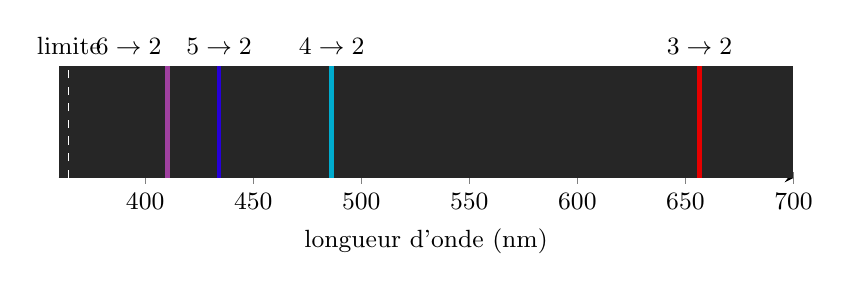
\begin{tikzpicture}
\begin{axis}[
  width=0.9\linewidth, height=3.0cm,
  xmin=360, xmax=700, ymin=0, ymax=1,
  axis x line=bottom, axis y line=none,
  xlabel={longueur d'onde (nm)}, xtick={400,450,500,550,600,650,700},
  tick label style={font=\small}, label style={font=\small},
  clip=false]
\fill[black!85] (axis cs:360,0) rectangle (axis cs:700,1);
% line positions: figdata/out/bachelor-1-hydrogen-levels-balmer.dat
\draw[line width=1.6pt, red!90!black] (axis cs:656.5,0) -- (axis cs:656.5,1);
\draw[line width=1.6pt, cyan!80!green] (axis cs:486.3,0) -- (axis cs:486.3,1);
\draw[line width=1.6pt, blue!70!violet] (axis cs:434.2,0) -- (axis cs:434.2,1);
\draw[line width=1.6pt, violet!75] (axis cs:410.3,0) -- (axis cs:410.3,1);
\draw[white, dashed] (axis cs:364.7,0) -- (axis cs:364.7,1);
\node[font=\small, anchor=south] at (axis cs:364.7,1.02) {limite};
\node[font=\small, anchor=south] at (axis cs:656.5,1.02) {$3\to2$};
\node[font=\small, anchor=south] at (axis cs:486.3,1.02) {$4\to2$};
\node[font=\small, anchor=south] at (axis cs:434.2,1.02) {$5\to2$};
\node[font=\small, anchor=south east] at (axis cs:412,1.02) {$6\to2$};
\end{axis}
\end{tikzpicture}

{\small Les raies de Balmer calculées par la formule de Rydberg
(longueurs d'onde dans le vide), sur le domaine visible. Les raies
suivantes se resserrent vers la limite de la série, à \qty{364.7}{nm},
dans l'ultraviolet.}
\end{omfigure}

\begin{history}[L'atome de Bohr, 1913]
En 1913, Niels Bohr, physicien danois de 28 ans qui travaillait à
Manchester, proposa que l'électron de l'hydrogène ne pouvait tourner
autour du noyau que sur certaines orbites, et que la lumière était
émise quand il sautait d'une orbite à une orbite inférieure. Son modèle
redonnait exactement les raies de Balmer, ainsi que la valeur de la
constante de Rydberg à partir de $h$, de $e$ et de la masse de
l'électron. Les orbites n'ont pas survécu à la mécanique quantique de
1925--1926, mais les niveaux quantifiés, si. Bohr reçut le prix Nobel
de physique en 1922.
\end{history}

\begin{omfigure}
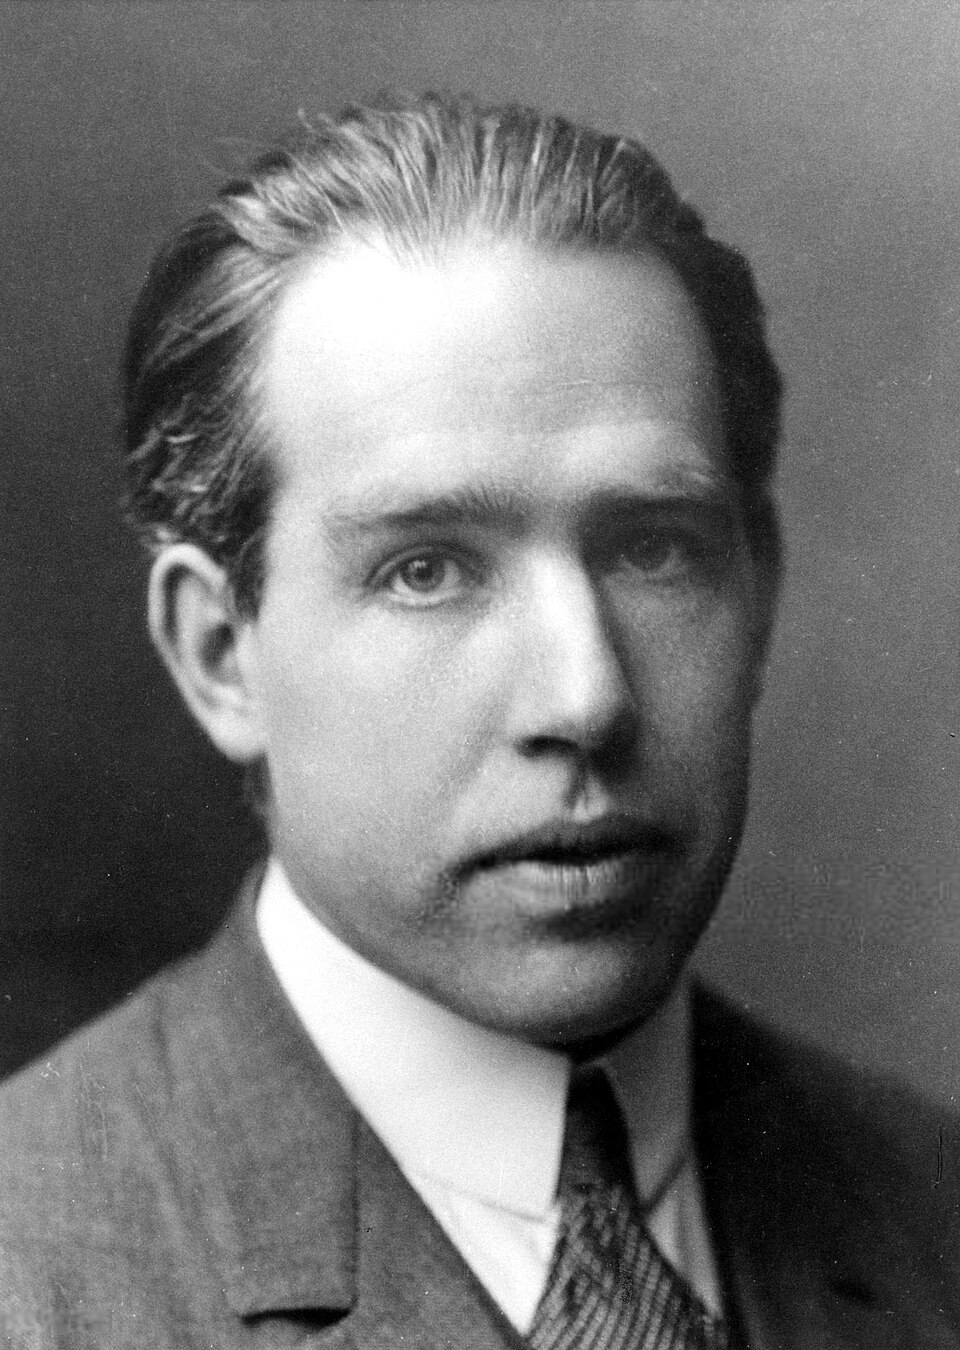
\includegraphics[width=0.26\linewidth]{images/book2/bohr.jpg}

{\small Niels Bohr (1885--1962), vers 1922.}
\end{omfigure}

\section{Quatre nombres quantiques}

Dans un atome à plusieurs électrons, les énergies ne sont plus données
par une formule unique, mais chaque électron reste décrit par un petit
ensemble d'entiers, ses nombres quantiques.

\begin{definition}[Nombres quantiques]\label{def:b1:quantum-numbers:quantum-number}
L'état d'un électron dans un atome est repéré par quatre nombres~:
\begin{itemize}
  \item le \emph{nombre quantique principal}\index{nombre quantique principal}
        $n = 1, 2, 3, \dots$, qui fixe pour l'essentiel l'énergie et la taille~;
  \item le \emph{nombre quantique azimutal}\index{nombre quantique azimutal}
        (ou nombre quantique secondaire) $l = 0, 1, \dots, n-1$, qui fixe
        la forme~; on note s, p, d, f les valeurs $l = 0, 1, 2, 3$~;
  \item le \emph{nombre quantique magnétique}\index{nombre quantique magnetique@nombre quantique magnétique}
        $m_l = -l, -l+1, \dots, l$, qui fixe l'orientation ($2l + 1$
        valeurs)~;
  \item le \emph{nombre quantique de spin}\index{nombre quantique de spin}
        $m_s = +\tfrac12$ ou $-\tfrac12$, propriété intrinsèque de
        l'électron, représentée par une flèche vers le haut ou vers le bas.
\end{itemize}
\end{definition}

\begin{definition}[Orbitale atomique, couche, sous-couche]\label{def:b1:quantum-numbers:orbital}
Une \emph{orbitale atomique}\index{orbitale atomique} est l'état à un
électron repéré par les trois nombres $(n, l, m_l)$~; on la représente
par une case, \omorbs{}. Les orbitales de même $n$ forment une
\emph{couche électronique}\index{couche electronique@couche électronique}~; celles de même $n$ et de même $l$ forment une
\emph{sous-couche}\index{sous-couche}, désignée par $n$ et par la lettre de $l$~:
2p est la sous-couche $n = 2$, $l = 1$, formée de trois orbitales
($m_l = -1, 0, 1$).
\end{definition}

\begin{remark}[Formes]\label{rem:b1:quantum-numbers:shapes}
Une orbitale s est sphérique~; une orbitale p a deux lobes le long d'un
axe, et les trois orbitales 2p sont dirigées selon $x$, $y$ et $z$. La
description mathématique de ces formes --- fonctions d'onde, parties
radiale et angulaire, surfaces nodales --- relève du volume de deuxième
année. Dans ce livre, une orbitale est une case qui contient au plus deux
électrons.
\end{remark}

\begin{proposition}[Capacité d'une sous-couche et d'une couche]\label{prop:b1:quantum-numbers:capacity}
Une \omterm{def:b1:quantum-numbers:orbital}{sous-couche} de nombre azimutal $l$ compte $2l + 1$ orbitales et
peut contenir $2(2l + 1)$ électrons~: 2 en s, 6 en p, 10 en d, 14 en f.
La couche $n$ compte $n^2$ orbitales et peut contenir $2n^2$ électrons.
\end{proposition}

\begin{proof}
Pour un $l$ donné, $m_l$ prend les $2l + 1$ valeurs de $-l$ à $l$, et
chaque orbitale contient deux électrons de spins opposés (\cref{prop:b1:quantum-numbers:pauli}
ci-dessous). Pour un $n$ donné, $l$ varie de $0$ à $n - 1$, donc le
nombre d'orbitales vaut
\[
  \sum_{l=0}^{n-1} (2l+1) = 2\,\frac{(n-1)n}{2} + n = n^2 ,
\]
et le nombre d'électrons $2n^2$~: 2, 8, 18, 32 pour $n = 1$ à 4.
\end{proof}

\begin{example}[La troisième couche]\label{ex:b1:quantum-numbers:third}
Pour $n = 3$~: $l = 0$ (3s, une orbitale), $l = 1$ (3p, trois
orbitales), $l = 2$ (3d, cinq orbitales, $m_l = -2, \dots, 2$)~: neuf
orbitales et au plus 18 électrons. Un électron 3d a par exemple les
nombres quantiques $(3, 2, -1, +\tfrac12)$.
\end{example}

\section{Établir une configuration}

\begin{definition}[Configuration électronique]\label{def:b1:quantum-numbers:configuration}
La \emph{configuration électronique}\index{configuration electronique@configuration électronique} d'un
atome ou d'un ion est la liste de ses \omterm{def:b1:quantum-numbers:orbital}{sous-couches} occupées, avec le
nombre d'électrons de chacune écrit en exposant~: $1\text{s}^2 2\text{s}^2
2\text{p}^4$ pour l'oxygène. Les électrons de $n$ le plus élevé, avec
ceux d'une \omterm{def:b1:quantum-numbers:orbital}{sous-couche} d ou f incomplètement remplie, sont les \emph{électrons
de valence}\index{electrons de valence@électrons de valence}~; les autres sont les \emph{électrons de
cœur}\index{electrons de coeur@électrons de cœur}. On abrège une configuration en écrivant entre
crochets celle du gaz noble qui précède~:
l'oxygène est $[\ce{He}]\,2\text{s}^2 2\text{p}^4$.
\end{definition}

Trois règles donnent la configuration de l'\omterm{def:b1:quantum-numbers:energy-level}{état fondamental}.

\begin{proposition}[Principe d'exclusion de Pauli]\label{prop:b1:quantum-numbers:pauli}
Deux électrons d'un même atome n'ont jamais les mêmes quatre nombres
quantiques. Une orbitale contient donc au plus deux électrons, et ceux-ci
ont alors des spins opposés~: \omorbs{ud}.
\end{proposition}
\admitted

\begin{proposition}[Règle de Klechkowski]\label{prop:b1:quantum-numbers:klechkowski}
Dans l'\omterm{def:b1:quantum-numbers:energy-level}{état fondamental} d'un atome neutre, les \omterm{def:b1:quantum-numbers:orbital}{sous-couches} se
remplissent par ordre de $n + l$ croissant et, à $n + l$ égal, par ordre
de $n$ croissant~:
\[
  1\text{s},\ 2\text{s},\ 2\text{p},\ 3\text{s},\ 3\text{p},\ 4\text{s},\
  3\text{d},\ 4\text{p},\ 5\text{s},\ 4\text{d},\ 5\text{p},\ 6\text{s},\
  4\text{f},\ 5\text{d},\ 6\text{p},\ 7\text{s},\ 5\text{f},\ 6\text{d},\
  7\text{p}.
\]
\end{proposition}
\admitted

\begin{remark}[Une règle empirique]\label{rem:b1:quantum-numbers:klech-empirical}
La règle de Klechkowski (dite aussi règle de Madelung) résume des
configurations observées~; ce n'est pas une loi~: elle décrit l'ordre
dans lequel les \omterm{def:b1:quantum-numbers:orbital}{sous-couches} se remplissent quand la charge du noyau
augmente. Dans un atome à plusieurs électrons, les électrons se
repoussent, de sorte que l'énergie d'une \omterm{def:b1:quantum-numbers:orbital}{sous-couche} dépend de $l$ autant
que de $n$~: un électron 4s, qui passe une partie de son temps près du
noyau, se retrouve sous le niveau 3d dans le potassium et le calcium.
\end{remark}

\begin{omfigure}
\begin{tikzpicture}[font=\small, x=1.25cm, y=0.72cm]
  \foreach \n in {1,...,7} {
    \foreach \l/\s in {0/s,1/p,2/d,3/f} {
      \pgfmathtruncatemacro\ok{(\l<\n) && (\n+\l<=8)}
      \ifnum\ok=1
        \node[draw=black!50, rounded corners=2pt, minimum width=0.85cm,
          minimum height=0.5cm, fill=white] (s\n\l) at (\l,-\n) {\n\s};
      \fi
    }
  }
  \begin{scope}[on background layer]
  \foreach \la/\na/\lb/\nb in {0/1/0/1, 0/2/0/2, 1/2/0/3, 1/3/0/4, 2/3/0/5,
      2/4/0/6, 3/4/0/7, 3/5/1/7} {
    \draw[-{Stealth}, omDef, thick, opacity=0.8]
      ($(\la,-\na)+(0.5,0.42)$) -- ($(\lb,-\nb)+(-0.5,-0.42)$);
  }
  \end{scope}
  \node[anchor=west, align=left, font=\small] at (4.0,-2.5) {suivre chaque flèche,\\puis la suivante\\à sa droite};
\end{tikzpicture}

{\small Le diagramme de Klechkowski. Les \omterm{def:b1:quantum-numbers:orbital}{sous-couches} de même $n + l$
sont sur une même diagonale~; parcourir les diagonales dans l'ordre
donne l'ordre de remplissage 1s, 2s, 2p, 3s, 3p, 4s, 3d, 4p, 5s, \dots}
\end{omfigure}

\begin{proposition}[Règle de Hund]\label{prop:b1:quantum-numbers:hund}
Lorsque les électrons d'une \omterm{def:b1:quantum-numbers:orbital}{sous-couche} peuvent se placer dans plusieurs
orbitales de même énergie, l'\omterm{def:b1:quantum-numbers:energy-level}{état fondamental} possède le plus grand
nombre de spins \emph{parallèles}~: les électrons occupent des orbitales
distinctes, spins vers le haut, avant qu'aucune orbitale ne reçoive deux
électrons.
\end{proposition}
\admitted

\begin{definition}[Électron célibataire]\label{def:b1:quantum-numbers:unpaired}
Un \emph{électron célibataire}\index{electron celibataire@électron célibataire} est un électron seul
dans son orbitale. Une espèce qui possède des électrons célibataires est
attirée par un aimant (elle est paramagnétique, propriété étudiée en
physique).
\end{definition}

\begin{method}[Écrire la configuration de l'état fondamental]\label{met:b1:quantum-numbers:configuration}
Pour écrire la configuration d'un atome de numéro atomique $Z$~:
\begin{enumerate}
  \item placer $Z$ électrons dans les \omterm{def:b1:quantum-numbers:orbital}{sous-couches} selon l'ordre de
        Klechkowski, en remplissant chaque \omterm{def:b1:quantum-numbers:orbital}{sous-couche} (2, 6, 10, 14)
        avant la suivante~;
  \item écrire le résultat par ordre de $n$ croissant (en regroupant 3d
        avec $n = 3$), et l'abréger avec le cœur du gaz noble qui
        précède~;
  \item pour la dernière \omterm{def:b1:quantum-numbers:orbital}{sous-couche}, incomplètement remplie, dessiner
        les cases et appliquer la règle de Hund pour compter les \omterm{def:b1:quantum-numbers:unpaired}{électrons
        célibataires}.
\end{enumerate}
\end{method}

\begin{example}[Carbone, azote, oxygène, fer]\label{ex:b1:quantum-numbers:examples}
La méthode donne, pour quatre atomes~:
\begin{center}
\begin{tabular}{lllc}
\hline
atome & configuration & dernière \omterm{def:b1:quantum-numbers:orbital}{sous-couche} & célibataires \\
\hline
\ce{C} ($Z = 6$) & $[\ce{He}]\,2\text{s}^2 2\text{p}^2$ & 2p~: \omorbs{u,u,} & 2 \\
\ce{N} ($Z = 7$) & $[\ce{He}]\,2\text{s}^2 2\text{p}^3$ & 2p~: \omorbs{u,u,u} & 3 \\
\ce{O} ($Z = 8$) & $[\ce{He}]\,2\text{s}^2 2\text{p}^4$ & 2p~: \omorbs{ud,u,u} & 2 \\
\ce{Fe} ($Z = 26$) & $[\ce{Ar}]\,3\text{d}^6 4\text{s}^2$ & 3d~: \omorbs{ud,u,u,u,u} & 4 \\
\hline
\end{tabular}
\end{center}
Pour le fer, l'ordre de Klechkowski remplit 4s ($Z = 19, 20$) avant 3d
($Z = 21$ à 30)~; la configuration s'écrit avec 3d en premier.
% ledger: gs:Fe
\end{example}

\begin{omfigure}
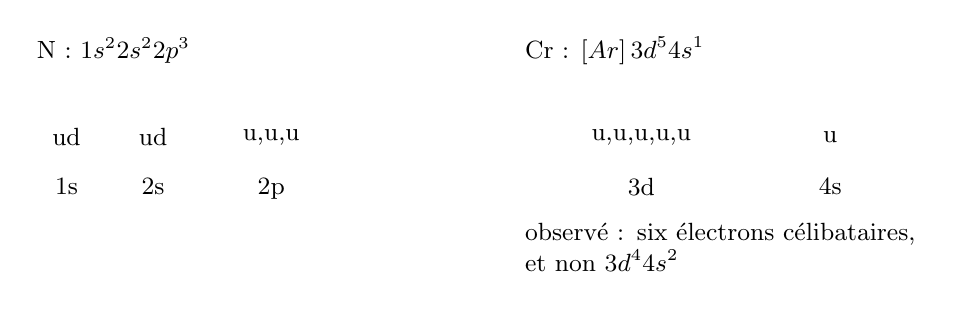
\begin{tikzpicture}[font=\small]
  \begin{scope}
    \node[anchor=west] at (0,2.4) {\ce{N}~: $1\text{s}^2 2\text{s}^2 2\text{p}^3$};
    \node at (0.5,1.3) {\omorbs{ud}}; \node[below] at (0.5,0.9) {1s};
    \node at (1.6,1.3) {\omorbs{ud}}; \node[below] at (1.6,0.9) {2s};
    \node at (3.1,1.3) {\omorbs{u,u,u}}; \node[below] at (3.1,0.9) {2p};
  \end{scope}
  \begin{scope}[xshift=6.2cm]
    \node[anchor=west] at (0,2.4) {\ce{Cr}~: $[\ce{Ar}]\,3\text{d}^5 4\text{s}^1$};
    \node at (1.6,1.3) {\omorbs{u,u,u,u,u}}; \node[below] at (1.6,0.9) {3d};
    \node at (4.0,1.3) {\omorbs{u}}; \node[below] at (4.0,0.9) {4s};
    \node[anchor=west, text width=5.0cm] at (0,-0.1) {observé~: six électrons célibataires, et non $3\text{d}^4 4\text{s}^2$};
  \end{scope}
\end{tikzpicture}

{\small Cases quantiques. Chaque case est une orbitale~; une flèche est
un électron et son spin. L'azote suit la règle de Hund~; le chrome est
l'une des exceptions de la \cref{prop:b1:quantum-numbers:exceptions}.}
\end{omfigure}

\section{Ions, exceptions et forme du tableau}

\begin{proposition}[Configurations des ions]\label{prop:b1:quantum-numbers:ions}
Un anion monoatomique a la configuration de l'atome complétée par les
électrons supplémentaires, placés aux rangs suivants de l'ordre de
Klechkowski~; un cation d'un élément des groupes principaux perd les
électrons de $n$ le plus élevé. Un cation d'un métal de transition perd
ses électrons $n$s \emph{avant} ses électrons
$(n-1)$d~: \ce{Fe^{2+}} est $[\ce{Ar}]\,3\text{d}^6$ et
\ce{Fe^{3+}} est $[\ce{Ar}]\,3\text{d}^5$, et non $[\ce{Ar}]\,3\text{d}^4
4\text{s}^2$.
% ledger: gs:Fe2+, gs:Fe3+
\end{proposition}
\admitted

\begin{remark}[Ordre de remplissage et ordre d'ionisation]\label{rem:b1:quantum-numbers:order}
La \omterm{def:b1:quantum-numbers:orbital}{sous-couche} 4s se remplit avant 3d dans le potassium et le calcium,
et pourtant elle se vide la première dans les ions des métaux de
transition. Il n'y a pas de contradiction~: l'ordre des énergies des
\omterm{def:b1:quantum-numbers:orbital}{sous-couches} change avec la charge du noyau et le nombre d'électrons, et
dans un atome ou un ion de métal de transition la \omterm{def:b1:quantum-numbers:orbital}{sous-couche} 3d est
sous 4s. La règle de Klechkowski ne décrit que les atomes neutres.
\end{remark}

\begin{proposition}[Deux exceptions dans la première série de transition]\label{prop:b1:quantum-numbers:exceptions}
Les configurations observées de l'\omterm{def:b1:quantum-numbers:energy-level}{état fondamental} du chrome et du cuivre sont
\[
  \ce{Cr}: [\ce{Ar}]\,3\text{d}^5 4\text{s}^1, \qquad
  \ce{Cu}: [\ce{Ar}]\,3\text{d}^{10} 4\text{s}^1 ,
\]
au lieu de $3\text{d}^4 4\text{s}^2$ et $3\text{d}^9 4\text{s}^2$
prévues par la règle de Klechkowski~: une \omterm{def:b1:quantum-numbers:orbital}{sous-couche} d à moitié remplie
ou pleine est particulièrement stable, et les niveaux 4s et 3d sont
proches.
% ledger: gs:Cr, gs:Cu
\end{proposition}

\begin{example}[Le cuivre et ses ions]\label{ex:b1:quantum-numbers:copper}
\ce{Cu} est $[\ce{Ar}]\,3\text{d}^{10} 4\text{s}^1$~; \ce{Cu+} est
$[\ce{Ar}]\,3\text{d}^{10}$, sans \omterm{def:b1:quantum-numbers:unpaired}{électron célibataire}~; \ce{Cu^{2+}}
est $[\ce{Ar}]\,3\text{d}^9$, avec un \omterm{def:b1:quantum-numbers:unpaired}{électron célibataire}. \ce{Zn^{2+}},
$[\ce{Ar}]\,3\text{d}^{10}$, n'en a aucun.
% ledger: gs:Cu+, gs:Cu2+, gs:Zn2+
\end{example}

\begin{proposition}[Configurations et tableau périodique]\label{prop:b1:quantum-numbers:table}
La période $n$ du tableau périodique commence avec le remplissage de
$n$s et se termine avec celui de $n$p. Les \omterm{def:b1:quantum-numbers:orbital}{sous-couches} remplies entre
les deux sont, d'après la règle de Klechkowski, $(n-2)$f et $(n-1)$d.
Les périodes comptent donc $2, 8, 8, 18, 18, 32, 32$ éléments, et les
gaz nobles ont $Z = 2, 10,
18, 36, 54, 86, 118$.
\end{proposition}

\begin{proof}
Les périodes 1 à 3 ne contiennent que $n$s (et $n$p pour $n \ge 2$)~:
$2$, puis deux fois $2 + 6 = 8$. Dans les périodes 4 et 5 s'ajoute
$(n-1)$d~: $2 + 10 + 6 =
18$. Dans les périodes 6 et 7 s'ajoute aussi $(n-2)$f~:
$2 + 14 + 10 + 6 = 32$. Les gaz nobles ferment chaque période~: $2$, $2 + 8 = 10$,
$18$, $18 + 18 = 36$, $54$, $54 + 32 = 86$, $118$.
\end{proof}

\begin{omfigure}
\omperiodictable[colour=blocks, legend]

{\small Le tableau périodique coloré selon la dernière \omterm{def:b1:quantum-numbers:orbital}{sous-couche} en
cours de remplissage~: les blocs s, p, d et f. La largeur de chaque bloc
est la capacité de sa \omterm{def:b1:quantum-numbers:orbital}{sous-couche}, 2, 6, 10 et 14.}
\end{omfigure}

\section{Exercices}

\begin{exercise}[$\star$]\label{exo:b1:quantum-numbers:1}
Parmi ces quadruplets $(n, l, m_l, m_s)$, lesquels peuvent décrire un
électron dans un atome~? Justifier chaque refus.
(a) $(2, 2, 0, +\tfrac12)$~; (b) $(3, 1, -1, -\tfrac12)$~;
(c) $(1, 0, 0, 0)$~; (d) $(4, 3, -3, +\tfrac12)$~; (e) $(3, 0, 1, -\tfrac12)$.
\end{exercise}

\begin{exercise}[$\star$]\label{exo:b1:quantum-numbers:2}
Combien d'orbitales, et au plus combien d'électrons, comptent les
\omterm{def:b1:quantum-numbers:orbital}{sous-couches} 3d, 4f et 5p, et la couche $n = 2$~?
\end{exercise}

\begin{exercise}[$\star$]\label{exo:b1:quantum-numbers:3}
Écrire les configurations de l'\omterm{def:b1:quantum-numbers:energy-level}{état fondamental} de \ce{O}, \ce{P},
\ce{K}, \ce{Ca} et \ce{Br} ($Z = 8, 15, 19, 20, 35$), sous forme
complète et abrégée, et donner le nombre d'\omterm{def:b1:quantum-numbers:configuration}{électrons de valence} de
chacun.
\end{exercise}

\begin{exercise}[$\star$]\label{exo:b1:quantum-numbers:4}
Dessiner les cases quantiques des \omterm{def:b1:quantum-numbers:orbital}{sous-couches} de valence de l'azote, du
soufre et du chlore, et compter leurs \omterm{def:b1:quantum-numbers:unpaired}{électrons célibataires}.
\end{exercise}

\begin{exercise}[$\star\star$]\label{exo:b1:quantum-numbers:5}
Donner les configurations de \ce{Na+}, \ce{Mg^{2+}}, \ce{Al^{3+}},
\ce{F-}, \ce{O^{2-}}, \ce{Cl-}, \ce{S^{2-}} et \ce{Ca^{2+}}. De quel gaz
noble chacun est-il isoélectronique~?
\end{exercise}

\begin{exercise}[$\star\star$]\label{exo:b1:quantum-numbers:6}
Écrire les configurations de \ce{Ti^{2+}}, \ce{Mn^{2+}}, \ce{Co^{2+}},
\ce{Ni^{2+}} et \ce{Zn^{2+}} ($Z = 22, 25, 27, 28, 30$) et donner le
nombre d'\omterm{def:b1:quantum-numbers:unpaired}{électrons célibataires} de chacun.
\end{exercise}

\begin{exercise}[$\star\star$]\label{exo:b1:quantum-numbers:7}
Calculer l'énergie et la longueur d'onde du photon émis lors de la
transition $4 \to 3$ de l'hydrogène. Dans quel domaine du spectre se
trouve-t-il~? Prendre $E_R = \qty{13.6}{eV}$ et $hc = \qty{1240}{eV.nm}$.
\end{exercise}

\begin{exercise}[$\star\star$]\label{exo:b1:quantum-numbers:8}
Identifier les éléments dont la configuration de l'\omterm{def:b1:quantum-numbers:energy-level}{état fondamental} se
termine par
(a) $3\text{s}^2 3\text{p}^4$~; (b) $4\text{s}^2 3\text{d}^{10} 4\text{p}^5$~;
(c) $5\text{s}^1$~; (d) $4\text{s}^2 3\text{d}^3$. Donner les quatre
nombres quantiques d'un électron de la dernière \omterm{def:b1:quantum-numbers:orbital}{sous-couche} de (a).
\end{exercise}

\begin{exercise}[$\star\star$]\label{exo:b1:quantum-numbers:9}
À l'aide de la règle de Klechkowski, expliquer pourquoi le
dix-neuvième électron du potassium va en 4s et non en 3d, et pourquoi la
période 3 compte 8 éléments et non 18.
\end{exercise}

\begin{exercise}[$\star\star\star$]\label{exo:b1:quantum-numbers:10}
Un ion à un seul électron, de noyau de charge $Ze$, a pour niveaux
$E_n = -Z^2 E_R/n^2$ (admis). Pour \ce{He+} ($Z = 2$), calculer
l'énergie d'ionisation et la longueur d'onde de la transition $2 \to 1$.
Comparer à l'hydrogène.
\end{exercise}

\begin{exercise}[$\star\star\star$]\label{exo:b1:quantum-numbers:11}
Dire si chaque configuration est celle d'un \omterm{def:b1:quantum-numbers:energy-level}{état fondamental}, d'un \omterm{def:b1:quantum-numbers:energy-level}{état
excité}, ou impossible, et pourquoi~: (a) $1\text{s}^2 2\text{s}^1 2\text{p}^1$~;
(b) $1\text{s}^2 2\text{s}^2 2\text{p}^7$~; (c) $1\text{s}^2 2\text{p}^2$~;
(d) $[\ce{Ne}]\,3\text{s}^2 3\text{p}^3$~; (e) $1\text{s}^3$.
\end{exercise}

\begin{exercise}[$\star\star\star$]\label{exo:b1:quantum-numbers:12}
Les sels de fer(III) sont plus fortement attirés par un aimant que les
sels de fer(II), et les sels de zinc pas du tout. Classer
\ce{Fe^{2+}}, \ce{Fe^{3+}}, \ce{Mn^{2+}}, \ce{Cu^{2+}} et \ce{Zn^{2+}}
par nombre d'\omterm{def:b1:quantum-numbers:unpaired}{électrons célibataires}, et expliquer l'observation en
admettant que l'attraction croît avec ce nombre.
\end{exercise}

\section{Problème~: les raies d'une lampe, et un monde à trois spins}

\begin{problem}[{Problème du week-end --- des quatre raies d'une lampe à
hydrogène à la longueur des périodes, et ce que serait le tableau si
l'électron avait trois états de spin}]
\label{pb:b1:quantum-numbers:1}
Prendre $E_R = \qty{13.6}{eV}$ et $hc = \qty{1240}{eV.nm}$ dans tout le
problème. Le domaine visible s'étend d'environ 400 à \qty{700}{nm}.

\medskip
\noindent\textbf{Partie I --- La lampe à hydrogène.}
\begin{enumerate}
  \item Calculer les énergies $E_1$ à $E_4$ de l'atome d'hydrogène.
  \item Calculer l'énergie et la longueur d'onde du photon émis lors de
        la transition $3 \to 2$. Quelle est sa couleur~?
  \item Calculer les longueurs d'onde des transitions $4 \to 2$, $5 \to 2$
        et $6 \to 2$.
  \item Pourquoi une lampe à hydrogène montre-t-elle exactement quatre
        raies visibles~? Calculer la longueur d'onde de $7 \to 2$ pour
        étayer la réponse.
  \item Calculer la limite de la série de Balmer.
  \item Calculer la longueur d'onde de la première raie de Lyman, $2 \to 1$.
        Pourquoi ne peut-on pas la voir~?
  \item Quelle est la plus grande longueur d'onde d'un photon capable
        d'ioniser un atome d'hydrogène dans son \omterm{def:b1:quantum-numbers:energy-level}{état fondamental}~?
\end{enumerate}

\medskip
\noindent\textbf{Partie II --- Dénombrer les états.}
\begin{enumerate}[resume]
  \item Donner les valeurs de $l$ et de $m_l$ pour $n = 3$~; combien
        d'orbitales la couche compte-t-elle~?
  \item Montrer que la couche $n$ contient $2n^2$ électrons~; appliquer
        à $n = 4$.
  \item Écrire l'ordre de Klechkowski jusqu'à 7p.
  \item En déduire la longueur des sept périodes.
  \item Expliquer pourquoi la \omterm{def:b1:quantum-numbers:orbital}{sous-couche} 3d n'apparaît pas dans la
        période 3.
  \item En déduire les numéros atomiques des gaz nobles.
\end{enumerate}

\medskip
\noindent\textbf{Partie III --- Les métaux de transition.}
\begin{enumerate}[resume]
  \item Écrire la configuration du fer ($Z = 26$) et dessiner ses cases
        3d. Combien d'\omterm{def:b1:quantum-numbers:unpaired}{électrons célibataires}~?
  \item Mêmes questions pour \ce{Fe^{2+}} et \ce{Fe^{3+}}. Lequel des
        deux a une \omterm{def:b1:quantum-numbers:orbital}{sous-couche} à moitié remplie~?
  \item La configuration observée du chrome est $[\ce{Ar}]\,3\text{d}^5
        4\text{s}^1$. La comparer à la prévision, et compter les
        \omterm{def:b1:quantum-numbers:unpaired}{électrons célibataires} dans chaque cas.
  \item Donner les configurations de \ce{Cu}, \ce{Cu+} et \ce{Cu^{2+}}.
  \item Lequel de \ce{Cu+} et de \ce{Cu^{2+}} possède des \omterm{def:b1:quantum-numbers:unpaired}{électrons
        célibataires}~?
  \item Parmi \ce{Sc^{3+}}, \ce{Ti^{3+}}, \ce{Mn^{2+}} ($Z = 21, 22, 25$),
        lequel a le plus d'\omterm{def:b1:quantum-numbers:unpaired}{électrons célibataires}~?
\end{enumerate}

\medskip
\noindent\textbf{Partie IV --- Un monde à trois spins.}
Imaginons un univers où $n$, $l$ et $m_l$ obéissent aux mêmes règles que
dans le nôtre, où l'ordre de Klechkowski est inchangé et le principe
d'exclusion s'applique, mais où le nombre de spin $m_s$ peut prendre
trois valeurs.
\begin{enumerate}[resume]
  \item Combien d'électrons une orbitale peut-elle contenir~? Une
        \omterm{def:b1:quantum-numbers:orbital}{sous-couche} de nombre $l$~? Une couche $n$~?
  \item Donner les capacités de 1s, 2s, 2p, 3s et 3p.
  \item Un gaz noble ferme une période avec une \omterm{def:b1:quantum-numbers:orbital}{sous-couche} p pleine
        (ou 1s pour la première). Quel est le numéro atomique du premier
        gaz noble~?
  \item Quel numéro atomique se comporterait comme un métal alcalin,
        avec un seul électron au-delà du premier gaz noble~?
  \item Combien d'éléments compterait la deuxième période~?
  \item Calculer le numéro atomique du deuxième gaz noble de ce monde.
\end{enumerate}
\end{problem}
